\section{Kinetic Theory}
\begin{frame}{Fokker-Planck Equation}
    \begin{equation}
        \dv{f}{t} + \mathbf{v}\cdot\pdv{f}{\mathbf{x}} + \frac{e}{m}(\mathbf{E+v\times B})\cdot\mathbf{v}\cdot\pdv{f}{\mathbf{v}} = \left(\pdv{f}{t}\right)_c
        \label{eq:fokker-planck-equation}
    \end{equation}

    In collisionless plasma, $(\partial_tf)_c=0$. The collisionless Fokker-Planck equation has another name called Vlasov equation.
\end{frame}

\begin{frame}{Landau Damping}
    \begin{itemize}
        \item Landau damping is predicted by kinetic theory.
        \item Damping exists for waves even in collisionless plasma as well.
        \item The damping comes from the interaction of wave with particles travelling at the phase velocity, $\omega/k$.
    \end{itemize}
    If we perturb the Vlasov equation, with $f = f_0 + f_1$ and $E = E_0 + E_1$, where the subscript 1 indicates that it is a perturbation quantity, we will have dispersion relation
    \begin{equation}
        \omega = \omega_p(1+3k^2\lambda_D^2)^{1/2} - i\left(\frac{\pi}{8}\right)^{1/2}\frac{\omega_p}{(k\lambda_D)^3}\exp\left[-\frac{1}{2}\left(\frac{1}{k^2\lambda_D^2}+3\right)\right]
        \label{eq:landau-damping}
    \end{equation}
\end{frame}

\begin{frame}{Collision}
    \begin{equation}
        \left(\pdv{f}{t}\right)_c = - \sum_\alpha\pdv{v_\alpha}(\expval{\Delta v_\alpha} f) + \frac{1}{2}\sum_{\alpha,\beta}\pdv[2]{}{v_\alpha}{v_\beta}\,(\expval{\Delta v_\alpha\Delta v_\beta}f)
        \label{eq:fokker-planck-collision-term}
    \end{equation}
    where $\expval{\Delta v_\alpha}$ is coefficient of dynamic friction and $\expval{\Delta v_\alpha\Delta v_\beta}$ diffusion tensor, and they are defined as
    \begin{align}
        \expval{\Delta v_\alpha}               & = \int \psi\Delta v_\alpha\dd{\Delta\mathbf{v}}/\Delta t \label{eq:coefficient-of-dynamic-friction} \\
        \expval{\Delta v_\alpha\Delta v_\beta} & = \int \psi\Delta v_\alpha\Delta v_\beta\dd{\Delta\mathbf{v}}/\Delta t \label{eq:diffusion-tensor}
    \end{align}
    The $\psi(\mathbf{v},\Delta\mathbf{v})$ is the probability of a particle with velocity $\mathbf{v}$ being scattered by $\Delta\mathbf{v}$ in the time $\Delta t$.
\end{frame}

\begin{frame}{Gyro-averaged Kinetic Equations}
    If the plasma phenomenon involves processes which are slow compared to the Larmor frequency and which vary slowly in space compared to the Larmor radius of the individual particle, then we can average the particle motion over the fast Larmor motion,
    \begin{equation}
        \dv{\bar{f}}{t} + \mathbf{v}_g\cdot\pdv{\bar{f}}{\mathbf{x}} + \left(e\mathbf{E}\cdot\mathbf{v}_g+\mu\pdv{B}{t}\right)\pdv{\bar{f}}{K} = \left(\pdv{\bar{f}}{t}\right)_c
        \label{eq:gyro-averaged-equation}
    \end{equation}
    where $\mu=mv_\perp^2/2B$ is the magnetic moment, $K=\frac{1}{2}mv^2$ is the kinetic energy, and
    \begin{equation}
        \mathbf{v}_g = v_\parallel\mathbf{b} + \frac{\mathbf{E\times B}}{B^2} + \frac{v_\parallel^2\mathbf{b\times (b\cdot\grad)b} + \mu\mathbf{b\times\grad}B}{\omega_c}
        \label{eq:guiding-center-velocity}
    \end{equation}
    is the guiding center velocity, and $\mathbf{b}=\mathbf{B}/B$ and $\omega_c = eB/m$.

    \begin{itemize}
        \item Gyro-averaged equation reduces 1 dimension compare to the Fokker-Planck equation.
        \item Not valid if the equilibrium possesses magnetic shear.
    \end{itemize}
\end{frame}

\begin{frame}{Fokker-Planck Equation for a Plasma}
    We first define the so-called Rosenbluth potentials,
    \begin{equation}
        \begin{aligned}
            H_j(\mathbf{v}) & = \left(1+\frac{m}{m_j}\right)\int \frac{f_j(\mathbf{v})}{\abs{\mathbf{v-v_j}}}\dd{\mathbf{v_j}} \\
            G_j(\mathbf{v}) & = \int f_j(\mathbf{v})\abs{\mathbf{v-v_j}}\dd{\mathbf{v_j}}
        \end{aligned}
        \label{eq:rosenbluth-potentials}
    \end{equation}
    The collision term, Eq.(\ref{eq:fokker-planck-collision-term}), can be written using these potentials,
    \begin{equation}
        \begin{aligned}
            \left(\pdv{f}{t}\right)_c = \sum_j \frac{e^2Z^2Z_j^2\ln\Lambda}{4\pi\epsilon_0^2m^2}
             & \left[ -\pdv{v_\alpha}\left(\pdv{H_j(\mathbf{v})}{v_\alpha} f(\mathbf{v})\right)\right.                                         \\
             & \left. +\frac{1}{2}\pdv[2]{}{v_\alpha}{v_\beta}\,\left(\pdv[2]{G_j(\mathbf{v})}{v_\alpha}{v_\beta} f(\mathbf{v})\right) \right]
        \end{aligned}
        \label{eq:collision-term-rosenbluth}
    \end{equation}
    Notice that $\expval{\Delta v_\alpha}$ and $\expval{\Delta v_\alpha\Delta v_\beta}$ can also be expressed using Rosenbluth potentials.
\end{frame}

\begin{frame}{Fokker-Planck Equation for a Plasma - Continued}
    We can also write the collision term as symmetric Landau integral form,
    \begin{equation}
        \left(\pdv{f}{t}\right)_c = \sum_j \frac{e^2Z^2Z_j^2\ln\Lambda}{4\pi\epsilon_0^2m^2} \pdv{v_\alpha}
        \int \left(  \frac{f_j(\mathbf{v_j})}{m} \pdv{f(\mathbf{v})}{v_\beta} - \frac{f(\mathbf{v})}{m_j} \pdv{f_j(\mathbf{v_j})}{v_{j\beta}} \right) u_{\alpha\beta} \dd{\mathbf{v_j}}
        \label{eq:collision-term-landau-integral}
    \end{equation}
    where $\mathbf{u=v-v_j}, u_{\alpha\beta}=(u^2\delta_{\alpha\beta} - u_\alpha u_\beta)/u^3$.

    In this way, once we have the initial distributions of each species, we can numerically solve the Fokker-Planck equation, Eq.(\ref{eq:fokker-planck-equation}).
\end{frame}

\begin{frame}{Fokker-Planck Coefficient under Maxwellian Distribution}
    Under Maxwellian distribution, we can calculate Rosenbluth potentials, Eq.(\ref{eq:rosenbluth-potentials}). The collision term $(\partial_t f)_c$, Eq.(\ref{eq:collision-term-rosenbluth}), becomes
    \begin{equation}
        \left(\pdv{f}{t}\right)_c = -\grad_v\cdot[\expval{\Delta\mathbf{v}_\parallel}f - \grad_\parallel(D_\parallel f) - D_\perp\grad_\perp f]
        \label{eq:collision-term-form}
    \end{equation}
    where $\grad_v$ means the divergence in velocity space, and the diffusion coefficients are
    \begin{align}
        D_\parallel & = \frac{1}{2}\expval{(\Delta v_\parallel)^2}                                                     \\
        D_\perp     & = \frac{1}{2}\expval{(\Delta v_{\perp\alpha})^2} = \frac{1}{2}\expval{(\Delta v_{\perp\beta})^2}
    \end{align}
\end{frame}

\begin{frame}{Relaxation Processes}
    The heat exchange time, $\tau_{ij}$, is defined by
    \begin{equation}
        \dv{T_i}{t} = \frac{T_j - T_i}{\tau_{ij}}
        \label{eq:heat-exchange-time-definition}
    \end{equation}
    For electrons and single charged ions the heat exhange time is
    \begin{equation}
        \tau_{ie} = \tau_{ei} = \frac{m_i}{2m_e}\tau_e
        \label{eq:heat-exchange-time-electron-ion}
    \end{equation}
    where $\tau_e$ is the electron collision frequency
    \begin{equation}
        \tau_e = 3(2\pi)^{3/2}\frac{\epsilon_0^2m_e^{1/2}T_e^{3/2}}{ne^4\ln\Lambda}
        \label{eq:electron-collision-frequency}
    \end{equation}
\end{frame}

\begin{frame}{Collision Times}
    If the temperature is in unit \unit{\kilo\eV}, then collision times (in \unit{\s}) are
    \begin{align}
        \tau_e & = 1.09\times10^{16}\frac{T_e^{3/2}}{n_iZ^2\ln\Lambda}                \\
        \tau_i & = 6.60\times10^{17}\frac{(m_i/m_p)^{1/2}T_i^{3/2}}{n_iZ^2\ln\Lambda}
    \end{align}
    Fig.

    The Coulomb logarithm is defined as $\ln\Lambda = \int_0^{\lambda_D} \frac{r\dd{r}}{r_0^2+r^2}$.
    \begin{itemize}
        \item electron-electron collisions
              \[ \ln\Lambda = 14.9-\frac{1}{2}\ln(n_e/10^20) + \ln T_e, \;\; \text{$T_e$ in \unit{\kilo\eV}} \]
        \item electron-ion collisions ($T\gtrsim 10$\unit{\eV})
              \[ \ln\Lambda = 15.2-\frac{1}{2}\ln(n_e/10^20) + \ln T_e, \;\; \text{$T_e$ in \unit{\kilo\eV}} \]
    \end{itemize}
\end{frame}

\begin{frame}{Collision Times - Figure}
    \begin{figure}
        \centering
        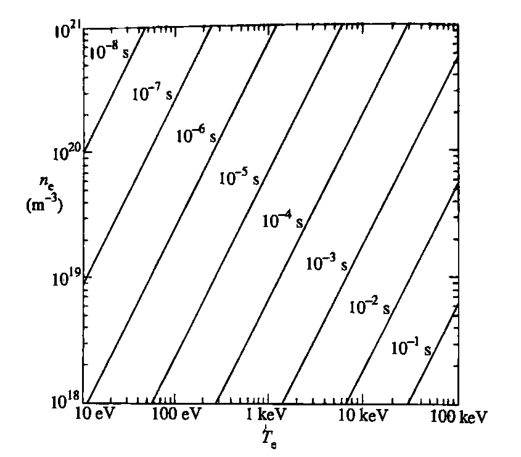
\includegraphics[width=0.6\textwidth]{figures/collision-time.png}
        \caption{Values of $\tau_e$ plotted against electron density and electron temperature.}
        \label{fig:collision-time}
    \end{figure}
\end{frame}

\begin{frame}{Resistivity}
    Resistivity can be defined by Ohm's law, $E=\eta j$.
    \begin{itemize}
        \item Singly charged ions (good for $B=0$ or in $B_\parallel$ direction):
              \begin{equation}
                  \eta_s = 0.51\frac{m_e^{1/2}e^2\ln\lambda}{3\epsilon_0^2(2\pi T_e)^{3/2}}, \;\;\;\text{$T_e$ in \unit{\kilo\eV}}
                  \label{eq:resistivity-singly-charged-ion}
              \end{equation}
        \item Plasma composed of several ion species,
              \[ \eta = Z_{eff}\eta_s, \;\; Z_{eff} = \frac{\sum_j n_jZ_j^2}{\sum_j n_jZ_j} \]
              It is obvious that $Z_{eff}=1$ for hydrogen plasma.
    \end{itemize}
    Worth to mention, resistivity in $B_\perp$ direction is almost twice of that in $B_\parallel$ direction,
    \[ \eta_\perp = \frac{m_e}{n_ee^2\tau_e} = 1.96\eta_\parallel \]
\end{frame}

\begin{frame}{Runaway Electrons - Simple Estimate}
    \begin{figure}
        \centering
        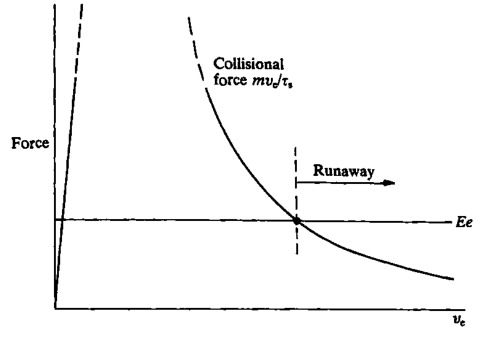
\includegraphics[width=0.5\textwidth]{figures/runaway-electrons.png}
        \caption{The electric field force, $Ee$, and the collisional force for an electron with a velocity $v_e$.}
        \label{fig:runaway-electrons}
    \end{figure}
    Fig.\ref{fig:runaway-electrons} shows that, electrons in the tail of velocity distribution might run away due to the presence of electric field. The critical velocity is
    \begin{equation}
        v_c^2 = \frac{3ne^3\ln\Lambda}{4\pi\epsilon_0^2m_eE} = 2.3\times10^{-4}\frac{n}{E}\; \unit{\m\tothe{2}\per\s\tothe{2}}, \;\; \ln\Lambda=17
        \label{eq:critical-velocity}
    \end{equation}
\end{frame}
